% Set up the document
\documentclass{article}

% Page size
\usepackage[
    letterpaper,]{geometry}

% Lines between paragraphs
\setlength{\parskip}{\baselineskip}
\setlength{\parindent}{0pt}

% Math
\usepackage{mathtools}
\usepackage{amssymb}
\usepackage{commath}

% Math notation macros
\newcommand{\R}{\mathbb{R}}
\newcommand{\Z}{\mathbb{Z}}

\def\*#1{\mathbf{#1}}
\def\ti#1{\tilde{#1}}
\newcommand{\dadvd}[2]{\dfrac{\text{D} #1}{\text{D} #2}} % advective derivative

\newcommand{\fS}{\mathcal{S}} % fancy S
\newcommand{\tphi}{\tilde{\phi}}
\newcommand{\nhat}{\mathbf{\hat{n}}}
\newcommand{\rhat}{\mathbf{\hat{r}}}
\newcommand{\thetahat}{\boldsymbol{\hat{\theta}}}
\newcommand{\xhat}{\mathbf{\hat{x}}}
\newcommand{\yhat}{\mathbf{\hat{y}}}
\newcommand{\zhat}{\mathbf{\hat{z}}}
\newcommand{\omegavec}{\boldsymbol{\omega}}

% Links
\usepackage{hyperref}

% Page numbers at top right
\usepackage{fancyhdr}
\pagestyle{fancy}
\fancyhf{}
\fancyhead[R]{\thepage}
\renewcommand\headrulewidth{0pt}

% Graphics
\usepackage{float}
\usepackage{graphicx}
\graphicspath{ {./img/} }

\begin{document}

\textbf{MATH 462 Assignment 9} \\
\textbf{Matt Wiens \#301294492} \\
\textbf{2020-03-28}

\textbf{101) It's a bore!} (3 pages + plot)
There is a further simplification to our surface wave theory of weeks 8
and 9 that applies when the wavelength of the waves is much greater than
the mean depth of the fluid. In 1D, the PDEs that describe this fluid
are
%
\begin{align*}
    h_t + (h u)_x = 0; \\
    u_t + u u_x + g h_x = 0
\end{align*}
%
for $u(x, t)$ and the fluid layer depth $h(x, t)$.

\textbf{i)} Following the presentation in lecture, derive the Riemann
invariant relations for these PDEs.

\textbf{ii)} Analyze a modification of the flow suggested by figure 3.17
in Acheson. The surfers shown below are surfing on a river and going
upstream! They can do this because there is a rising tide at the mouth
of the river (say, at $x = 0$). Take the initial conditions on the river
($x > 0$) to be constant height $h_0$ and seaward flow velocity $-u_0 <
0$. For simplicity, consider the incoming tidal seawater (salty) as an
accelerating moving wall with velocity $x^\prime_s(t) = u_s = -u_0 +
\alpha t$. Again, following the presentation in lecture, derivate the
equation for the characteristics that are generated by the moving wall
boundary. As the upstream conditions are constant, these characteristics
can be shown to be straight lines.

Make a plot of these characteristics in the $x-t$ plane. Use the
following values for the constants: $c_0 = \sqrt{g h_0} = 1$, $\alpha =
c_0 / 3$, $u_0 = c_0 / 4$.

\newpage

\textbf{Solution}

\textbf{i)} Following what we did in lecture we can write our system as
%
\begin{equation*}
    \begin{pmatrix}
        h \\
        u
    \end{pmatrix}_t
    +
    \begin{pmatrix}
        u & h \\
        g & u
    \end{pmatrix}
    \begin{pmatrix}
        h \\
        u
    \end{pmatrix}_x
    = \*0
    .
\end{equation*}
%
Then, writing
%
\begin{equation*}
    \lambda = u \pm c
\end{equation*}
%
with
%
\begin{equation*}
    c = \sqrt{g h}
    ,
\end{equation*}
%
as in lectures we have
%
\begin{equation*}
    (\lambda - u)^2 = g h = c^2
    .
\end{equation*}
%
This lets us identify the left eigenvectors $\*w_1$ (I did this using
Maple) as
%
\begin{equation*}
    \*w_1^T
    = \del{\pm \sqrt{\frac{h}{g}}, 1}
    = \del{\pm \frac{h}{c}, 1}
    .
\end{equation*}
%
Left-multiplying our above system with these eigenvectors gives us
%
\begin{equation}
    \del{\pm \frac{h}{c} \, h_t + u_t} + (u \pm c) \del{\pm \frac{h}{c} \, h_x + u_x} = 0
    \label{eq:1-i-raw}
    .
\end{equation}
%
Noting that
%
\begin{equation*}
    \frac{h}{c}\, h_t
    = \frac{c}{g} \del{\frac{c^2}{g}}_t
    = \frac{2}{g^2} c^2 \, c_t
    = \del{\frac{2}{3 g^2} c^3}_t
    ,
\end{equation*}
%
we can write~\eqref{eq:1-i-raw} as
%
\begin{equation*}
    \del{\pm \frac{2}{3 g^2} c^3 + u}_t + (u \pm c) \del{\pm \frac{2}{3 g^2} c^3 + u}_x = 0
\end{equation*}
%
and hence identify the Riemann invariants $R^\pm$ as
%
\begin{equation*}
    R^\pm = \pm \frac{2}{3 g^2} c^3 + u
    .
\end{equation*}

\textbf{ii)} So now we're given the velocity $u_s = - u_0 + \alpha t$, and hence our
characteristics become
%
\begin{equation*}
    R^\pm = \pm \frac{2}{3 g^2} c^3 + \alpha t - u_0
    .
\end{equation*}
%
As we did in lecture, we can consider the ``undisturbed fluid'' (UF) and
``disturbed fluid'' (DF) regions separately. The UF region, where $x >
(-u_0 + c_0) t$, we just use our initial values (as was diagrammatically
argued in lectures), so
%
\begin{equation*}
    R^\pm_{\text{UF}} = \pm \frac{2}{3 g^2} c^3 - u_0
    .
\end{equation*}
%
Here, because $u \pm c$ is constant, the characteristics must be
straight lines. Note that the left-moving characteristics $R^-$ have the
above value \textit{everywhere} in both regions, since each of these
intersect the line $t = 0$.

For the DF region, we consider $-u_0 t + \frac{\alpha}{2} t^2 < x < (-
u_0 + c_0) t$. Here for the $R^-$ curves we have that the
characteristics have derivative $u - c$, so these are will generally not
be straight lines. For the $R^+$ characteristics, note that we can
express the $u + c$ as a function of $R^+$ and $R^-$ by inverting our
above equations for $R^\pm$ (this works in Maple but the formulas are a
little complicated). Hence the equation of motion for $R^+$ is
%
\begin{equation*}
    (R^+)_t + c(R^+, R^-) (R^-)_x = 0
    .
\end{equation*}
%
Since $R^-$ is constant everywhere and $R^+$ is constant along $R^+$
characteristics, $c(R^+, R^-)$ is constant along $R^+$ characteristics
and hence these characteristics are straight lines in the DF region (in
addition to being straight lines in the UF region). Using that $R^-$
characteristics are constant in both regions, we have that
%
\begin{equation*}
    - \frac{2}{3 g^2} c_0^3 - u_0 = - \frac{2}{3 g^2} c^3 + u
\end{equation*}
%
or
%
\begin{equation*}
    c = \frac{1}{2} \del{8 c_0^3 + 12 u g^2 + 12 u_0 g^2}^\frac{1}{3}
    .
\end{equation*}
%
Hence the slopes of the $R^+$ characteristics are given by $u_w + c(u_w)$
where $u_w = -u_0 + \alpha t_w$ is the velocity of the characteristic
starting at $x_w, t_w$.

Plotted on the following page are the $R^+$ characteristics for $g =
9.81$, $h_0 = 0.25$, $c_0 = \sqrt{g h_0}$, $\alpha = c_0 / 3$, and $u_0
= c_0 / 4$. The curve of the ``oncoming wave'' is plotted in blue and
the line $x = (-u_0 + c_0) t$ is plotted in red.

\begin{figure}
    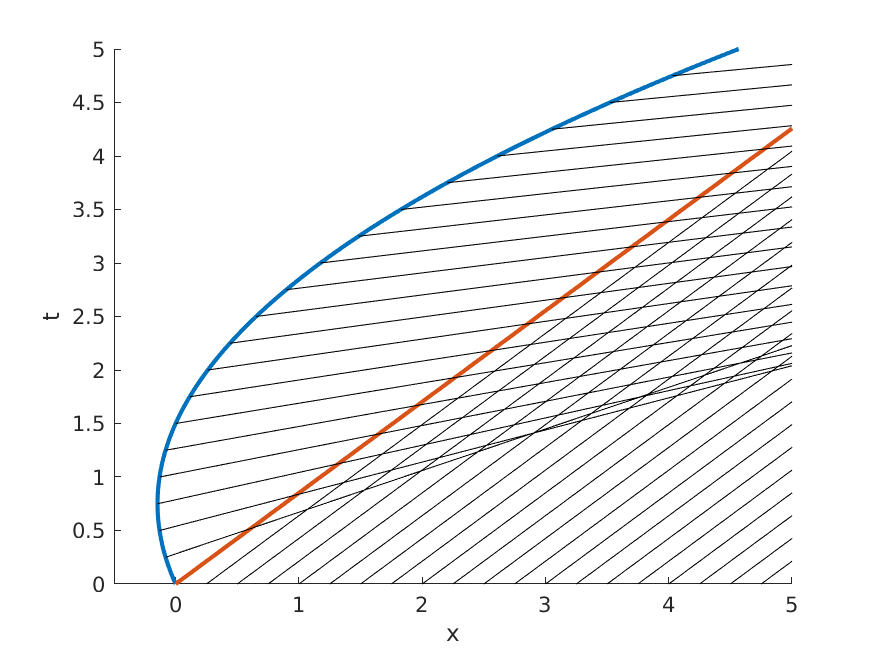
\includegraphics[width=40em]{as09fig1}
    \centering
\end{figure}

\newpage

\textbf{202) Milne-Thomson Circle Theorem}
So currently there isn't much on Canvas about this question, but I think
it's the most interesting one, so I'll do what I can here.

\textbf{The claim}

The claim here is that for any potential flow $\Phi$ whose singular
points lie in $|z| > a$, (i) we can preserve all singularities for $|z|
> a$, and (ii) have $|z| = a$ as a streamline with a new complex
potential
%
\begin{equation*}
    \Phi_{mt}(z) = \Phi(z) + \del{\Phi \del{\frac{a^2}{z^*}}}^*
    .
\end{equation*}

\textbf{Proof}

For notational convenience, denote
%
\begin{equation*}
    \ti{\Phi}(z) \coloneqq \del{\Phi \del{\frac{a^2}{z^*}}}^*
    .
\end{equation*}
%
To prove (i) we essentially need to show that there are no singularities
of $\ti\Phi$ after $|z| > a$. Suppose that $z$ is a singular point of
$\ti\Phi$. Then
%
\begin{equation*}
    \ti\Phi(z) = \del{\Phi \del{\frac{a^2}{z^*}}}^*
\end{equation*}
%
is a singularity. But since all singularities of $\Phi$ lie in $|z| >
a$ this implies that
%
\begin{equation*}
    \envert{\frac{a^2}{z^*}} > a
    ,
\end{equation*}
%
which further implies that $|z| < a$. Hence all singular points of
$\ti\Phi$ lie in $|z| < a$ and thus the singularities for $|z| > a$ for
$\Phi_{mt}$ are the same as for $\Phi$.

Now we'll prove (ii), which states that $|z| = a$ is a streamline. To
see this note that we can square the above expression to yield $z z^* =
a^2$. Then we have that, on $|z| = a$
%
\begin{equation*}
    \ti\Phi(z)
        = \del{\Phi \del{\frac{a^2}{z^*}}}^*
        = \del{\Phi \del{\frac{(z z^*)}{z^*}}}^*
        = \del{\Phi(z)}^*
\end{equation*}
%
and thus (still on the $|z| = a$)
%
\begin{equation*}
    \Phi_{mt}(z) = \Phi(z) + \ti\Phi(z) = \Phi(z) + \del{\Phi(z)}^* = 2 \Re\del{\Phi(z)}
    .
\end{equation*}
%
Therefore $\Phi_{mt}(z)$ is purely real on the circle, and therefore
$\psi_{mt} = 0$ on $|z| = a$ and hence this is a streamline.

\textbf{An example}

Let's just try this with a very simple example. Consider the potential
flow $\Phi(z) = z$. Here we have $\phi = x$ and $\psi = y$. This gives
us the familiar flow shown in Figure~\ref{fig:mt-1}.
%
\begin{figure}[!ht]
    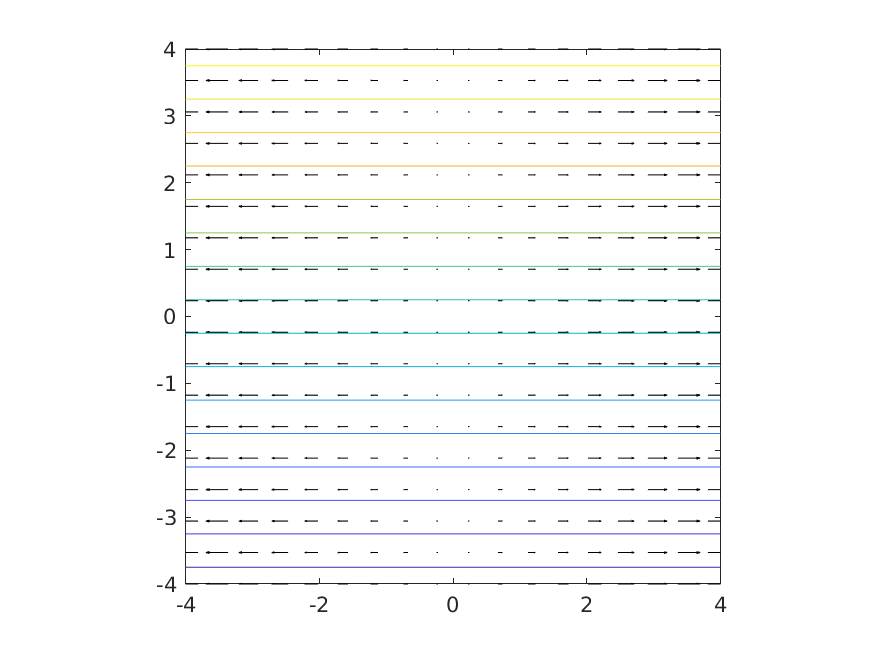
\includegraphics[width=35em]{as09fig2}
    \centering
    \caption{Flow generated from $\Phi$}
    \label{fig:mt-1}
\end{figure}

Now let's see what happens when we apply Milne-Thomson, taking $a = 2$. Then we have
%
\begin{equation*}
    \Phi_{mt} = z + \frac{4}{z}
    ,
\end{equation*}
%
and hence
%
\begin{align*}
    \phi_{mt} &= x + \frac{4 x}{x^2 + y^2}, \\
    \psi_{mt} &= y - \frac{4 y}{x^2 + y^2}
    .
\end{align*}
%
The resulting flow is plotted below in Figure~\ref{fig:mt-2}. In this
figure, the streamline $\psi = 0$ is plotted below in black, and we can
see that it aligns perfectly with the circle $|z| = 2$. Note also that
velocity quivers at $|z| < 1$ where not plotted, due to their large
magnitude near the origin.
%
\begin{figure}[!ht]
    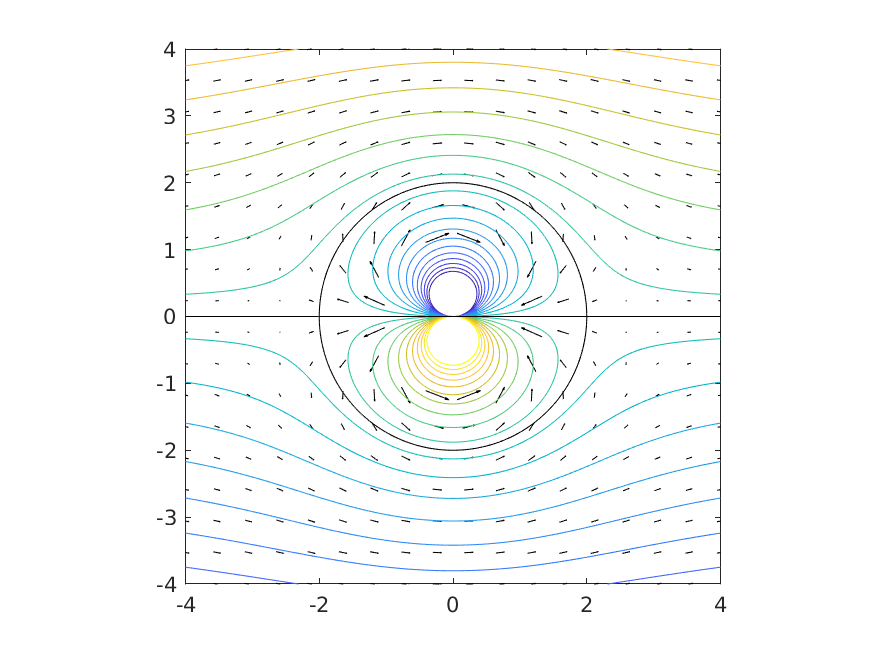
\includegraphics[width=35em]{as09fig3}
    \centering
    \caption{Flow generated from $\Phi_{mt}$}
    \label{fig:mt-2}
\end{figure}

\textbf{Thoughts}

Having done the above example I have a better sense of what
Milne-Thomson \textit{does}. Essentially it's useful if we want to embed
some immovable circular object in an arbitrary flow (given that there
are no singularities where we want to place the circle. This could
probably be extended to approximate arbitrary shapes, by using many
circles to approximate a shape and applying Milne-Thomson successively
(or all at once?).

\end{document}
